\documentclass[10pt,a4paper,twocolumn]{article}
\usepackage[utf8]{inputenc}
\usepackage[T1]{fontenc}
\usepackage{lmodern}
\usepackage[french]{babel}
\usepackage[margin=1.65cm,top=1.6cm,bottom=1.7cm,columnsep=0.6cm]{geometry}
\usepackage{graphicx,booktabs,amsmath,amssymb,multirow,array,caption,float,microtype,enumitem,url,xcolor}
\usepackage[hidelinks]{hyperref}
\captionsetup{font=small,labelfont=bf,skip=3pt}
\setlength{\textfloatsep}{8pt plus 2pt minus 2pt}
\setlength{\floatsep}{8pt plus 2pt minus 2pt}
\setlength{\intextsep}{8pt plus 2pt minus 2pt}
\renewcommand{\arraystretch}{1.05}
\setlength{\tabcolsep}{3.2pt}
\usepackage{titlesec}
\titleformat{\section}{\normalfont\large\bfseries}{\thesection}{0.6em}{}
\titlespacing*{\section}{0pt}{8pt plus 2pt minus 2pt}{3pt}
\titlespacing*{\subsection}{0pt}{5pt plus 2pt minus 1pt}{2pt}
\titleformat{\paragraph}[runin]{\normalfont\normalsize\bfseries}{}{0pt}{}
\titlespacing*{\paragraph}{0pt}{2.5pt plus 1pt minus 1pt}{0.55em}
\titleformat{\subsection}{\normalfont\normalsize\bfseries}{\thesubsection}{0.5em}{}
\setlength{\parskip}{0pt}

% ---- Auteurs : à compléter ------------------------------------------------
\newcommand{\AuteurNom}{[Prénom NOM]}
\newcommand{\AuteurAffil}{[Établissement / Filière]}
\newcommand{\AuteurMail}{[adresse e-mail]}

\title{\vspace{-0.6cm}\textbf{Optimisation d'hyperparamètres d'une forêt aléatoire pondérée\\ pour la détection de la sévérité de la dépression\\ à partir de biomarqueurs mitochondriaux}\\[3pt]
\large Reproduction de Bader \emph{et al.} (2024), validation croisée imbriquée\\ et audit de fuite de données}
\author{\AuteurNom\\ \small \AuteurAffil\\ \small \texttt{\AuteurMail}}
\date{}

\begin{document}

\twocolumn[
\begin{@twocolumnfalse}
\maketitle
\vspace{-0.9cm}
\begin{center}\begin{minipage}{0.92\textwidth}\small
\textbf{Résumé.} La sévérité de la dépression se mesure par le score PHQ-9, et des biomarqueurs sanguins pourraient aider à la suivre. Nous reproduisons le protocole de Bader \emph{et al.} (2024), fondé sur une forêt aléatoire pondérée (WRF), sur 2\,621 observations décrites par trois biomarqueurs mitochondriaux et neuf variables cliniques, puis nous l'améliorons par un pipeline complet d'optimisation d'hyperparamètres (GridSearchCV, RandomizedSearchCV, recherche bayésienne Optuna) sous validation croisée stratifiée. Dix modèles sont comparés avant et après optimisation, en classification binaire et à quatre classes, avec une validation croisée imbriquée $5\times 2$ et des tests de Wilcoxon, de Nadeau--Bengio et de Friedman--Conover. Dans le protocole de l'article, la RF atteint une AUC de test de 0,93 (binaire) et 0,90 (quatre classes), et la WRF optimisée 0,93 ; mais l'optimisation ne profite significativement qu'à KNN, SVM et ANN ($+0{,}04$ à $+0{,}12$ d'AUC), pas aux forêts. Un audit montre que 67 à 85\,\% des valeurs de biomarqueurs sont dupliquées entre lignes et presque parfaitement alignées sur la classe de sévérité : sur les 228 lignes sans doublon, l'AUC chute à 0,60--0,72 et l'optimisation ne procure plus aucun gain (RF : $-0{,}03$). Les scores élevés semblent donc refléter une fuite de données plutôt qu'un signal biologique, ce qui conditionne toute conclusion.


\smallskip
\textbf{Mots-clés :} forêt aléatoire pondérée ; optimisation d'hyperparamètres ; GridSearchCV ; validation croisée stratifiée ; fuite de données ; PHQ-9.
\end{minipage}\end{center}
\vspace{0.2cm}
\end{@twocolumnfalse}
]

\section{Introduction}

\subsection{Contexte général}
La dépression majeure est l'une des premières causes d'incapacité dans le monde : environ 280 millions de personnes en seraient atteintes, soit près de 5\,\% des adultes \cite{bader2024,hidaka2012}. Son évaluation clinique repose sur des questionnaires, dont le \emph{Patient Health Questionnaire} (PHQ-9) \cite{kroenke2001}, qui convertit les symptômes en un score gradué selon la sévérité. En parallèle, plusieurs travaux relient la dépression à un déséquilibre redox (stress oxydatif) \cite{black2015} et à une dysfonction mitochondriale. Des biomarqueurs sanguins pourraient ainsi compléter le questionnaire et aider les cliniciens à suivre la progression de la maladie ; l'apprentissage automatique est l'outil naturel pour les combiner avec les facteurs socio-démographiques et cliniques.

\subsection{Problématique}
Bader \emph{et al.} \cite{bader2024} montrent qu'une forêt aléatoire pondérée (\emph{weighted random forest}, WRF) atteint une AUC macro de 0,91 pour classer quatre niveaux de sévérité du PHQ-9 chez 830 participants. Trois verrous subsistent toutefois.
\begin{enumerate}[leftmargin=*,itemsep=0pt,topsep=2pt]
\item \textbf{Déséquilibre.} Les classes modérée et sévère représentent ensemble moins de 4\,\% des observations.
\item \textbf{Optimisation des hyperparamètres.} Le corps de l'article indique seulement qu'une validation croisée à 5 plis avec \emph{grid search} est menée sur l'ensemble d'entraînement ; les espaces de recherche ne sont pas décrits et le gain apporté par l'optimisation n'est pas quantifié (pas de comparaison « avant/après »).
\item \textbf{Fiabilité de l'évaluation.} Le jeu de données provient de visites répétées d'une même cohorte et de valeurs imputées \cite{bader2024,jelinek2014} : dans ces conditions un découpage aléatoire peut laisser fuiter de l'information entre apprentissage et test \cite{kaufman2012}.
\end{enumerate}

\subsection{Objectifs}
Nous cherchons (i) à \textbf{reproduire} le protocole de l'article source (six classifieurs, variantes pondérées et SMOTE, découpage 70/30, validation croisée à 5 plis, tests de Friedman et de Conover) sur le jeu de données fourni ; (ii) à \textbf{améliorer} ces résultats en mettant en place un pipeline complet d'optimisation d'hyperparamètres (\texttt{GridSearchCV}, \texttt{RandomizedSearchCV} et une recherche bayésienne avec Optuna) sous validation croisée stratifiée, et à comparer les performances \textbf{avant et après optimisation} ; (iii) à \textbf{évaluer} cette amélioration de façon statistiquement rigoureuse et critique.

\subsection{Contributions}
\begin{itemize}[leftmargin=*,itemsep=0pt,topsep=2pt]
\item Un pipeline reproductible (graines fixées, versions des bibliothèques, code fourni) comparant dix modèles : les six classifieurs de l'article, WLR, WRF, RF-SMOTE, et un modèle ajouté, le \emph{gradient boosting} pondéré (WHGB).
\item Une comparaison \textbf{avant/après optimisation} de la grille exhaustive, de la recherche aléatoire et de la recherche bayésienne (TPE) à budget comparable, avec coût de calcul.
\item Une \textbf{validation croisée imbriquée} $5\times 2$ fournissant des scores appariés, soumis à des tests de Wilcoxon, de Student corrigé \cite{nadeau2003} et de Friedman/Conover.
\item Un \textbf{audit de fuite de données} du fichier fourni, qui conduit à distinguer deux régimes d'analyse (« complet » et « propre ») et modifie profondément la lecture des résultats.
\end{itemize}

\subsection{Organisation de l'article}
La section~2 présente l'état de l'art, la section~3 les fondements théoriques, la section~4 la méthodologie (données, baseline, stratégie d'amélioration, protocole). La section~5 rapporte les expérimentations et leur discussion, et la section~6 conclut. Les espaces de recherche et des tableaux complémentaires figurent en annexe.

\section{État de l'art}

\subsection{Concepts clés}
\paragraph{Forêt aléatoire.} Une forêt aléatoire (RF) agrège des arbres de décision entraînés sur des échantillons bootstrap, chaque scission ne considérant qu'un sous-ensemble aléatoire de variables \cite{breiman2001}. Ses hyperparamètres déterminants sont le nombre d'arbres, la profondeur maximale, la taille minimale des feuilles et le nombre de variables testées par scission.

\paragraph{Gestion du déséquilibre.} Deux familles s'opposent : le \emph{rééchantillonnage}, notamment SMOTE qui synthétise des exemples minoritaires par interpolation \cite{chawla2002}, et la \emph{pondération des classes}, qui pénalise davantage les erreurs sur les classes rares dans la fonction de coût ou le critère d'impureté (WRF \cite{chen2004,zhang2016}, régression logistique pondérée WLR \cite{maalouf2014}).

\paragraph{Optimisation d'hyperparamètres (HPO).} La recherche sur grille explore exhaustivement un produit cartésien de valeurs ; la recherche aléatoire tire les configurations dans des distributions et se montre plus efficace lorsque peu d'hyperparamètres sont influents \cite{bergstra2012} ; la recherche bayésienne (estimateur TPE) concentre les essais sur les régions prometteuses \cite{bergstra2011,akiba2019}.

\paragraph{Validation.} La validation croisée stratifiée à $K$ plis conserve les proportions de classes \cite{kohavi1995}. Lorsque la même validation sert à choisir les hyperparamètres \emph{et} à estimer la performance, l'estimation est optimiste ; la validation croisée imbriquée corrige ce biais \cite{cawley2010}. Enfin, la \emph{fuite de données} (\emph{leakage}) --- toute information de la cible ou de lignes de test disponible à l'entraînement --- gonfle artificiellement les scores \cite{kaufman2012}.

\subsection{Travaux antérieurs}
\textbf{Article source.} Bader \emph{et al.} \cite{bader2024} étudient 830 participants (dernière visite de chaque patient, parmi 2\,621 observations), décrits par 14 variables : cinq biomarqueurs de stress oxydatif (8-isoprostane, 8-OHdG, GSH, GSSG, rapport GSH/GSSG), l'haplotype ACE et huit variables cliniques ou démographiques. Six classifieurs (LR, RF, KNN, SVM, NB, ANN) sont comparés en classification binaire (PHQ-9\,$>4$) et à quatre classes (0--4, 5--13, 14--20, $\geq 21$), avec découpage 70/30 et validation croisée à 5 plis avec \emph{grid search}. La RF obtient une AUC de 0,84 (binaire) et 0,88 (quatre classes) avec toutes les variables ; la WRF atteint 0,91 à quatre classes, devant WLR et RF-SMOTE, la différence étant jugée significative par les tests de Friedman et de Conover. Le glutathion réduit (GSH) est la variable la plus importante par permutation.

\textbf{Approches concurrentes.} Sau et Bhakta \cite{sau2017} obtiennent une AUC de 0,94 avec une RF sur 520 personnes âgées à partir de variables socio-démographiques et de santé ; Priya \emph{et al.} \cite{priya2020} trouvent que la RF offre la meilleure exactitude sur des données déséquilibrées (échelle DASS-21) ; Zulfiker \emph{et al.} \cite{zulfiker2021} combinent SMOTE et AdaBoost (AUC de 0,96). Ces travaux rapportent surtout des performances, rarement l'espace de recherche des hyperparamètres ni la protection contre la fuite de données.

\subsection{Positionnement}
Notre travail \emph{reproduit le protocole} de \cite{bader2024} sur un jeu de données distinct (biomarqueurs mitochondriaux) puis \emph{l'améliore sur trois plans} : (a) une HPO explicite et comparée (grille, aléatoire, bayésienne), avec espaces publiés et coûts mesurés ; (b) une inférence statistique sur scores appariés issus d'une validation imbriquée, avec correction pour la dépendance entre plis \cite{nadeau2003} ; (c) un audit de fuite de données, absent des travaux précités, qui conditionne l'interprétation de tous les gains.

\section{Fondements théoriques}

\subsection{Méthodes de base}
\paragraph{Forêt aléatoire.} Soit un échantillon d'apprentissage $\{(x_i,y_i)\}_{i=1}^{n}$ avec $y_i\in\{1,\dots,K\}$. Chaque arbre $b\in\{1,\dots,B\}$ est entraîné sur un échantillon bootstrap, et chaque scission choisit, parmi $m$ variables tirées au hasard, celle qui minimise l'impureté de Gini $G=1-\sum_{k}p_k^{2}$. La probabilité prédite est la moyenne des probabilités des feuilles :
\begin{equation}
\hat p(k\mid x)=\frac1B\sum_{b=1}^{B}\hat p_b(k\mid x),\qquad \hat y=\arg\max_k \hat p(k\mid x).
\end{equation}

\paragraph{Pondération des classes.} Chaque classe $j$ reçoit le poids de l'équation~(9) de \cite{bader2024} (identique à l'option \texttt{class\_weight='balanced'} de scikit-learn)~:
\begin{equation}
W_j=\frac{n}{K\,n_j},
\label{eq:weights}
\end{equation}
où $n_j$ est l'effectif de la classe $j$. Dans la WRF, les proportions utilisées pour l'impureté et pour le vote des feuilles deviennent $\tilde p_k=W_k n_k/\sum_j W_j n_j$ ; dans la WLR, la perte devient $-\sum_i W_{y_i}\log\hat p(y_i\mid x_i)$ plus la pénalité $\ell_1$ ou $\ell_2$.

\paragraph{SMOTE.} Pour un exemple minoritaire $x_i$ et l'un de ses $k$ plus proches voisins minoritaires $x_{nn}$, SMOTE crée $x_{\text{new}}=x_i+\lambda\,(x_{nn}-x_i)$, avec $\lambda\sim\mathcal U(0,1)$ \cite{chawla2002}.

\paragraph{Autres classifieurs.} LR (régression logistique), KNN, SVM à noyau RBF (problème dual avec pénalité $C$), Bayes naïf gaussien (NB) et perceptron multicouche (ANN, activation ReLU, 350 itérations) complètent la comparaison, comme dans \cite{bader2024} ; WHGB est un \emph{gradient boosting} par histogrammes avec les poids de l'éq.~\eqref{eq:weights}.

\subsection{Métriques d'évaluation}
Avec $TP,FP,FN,TN$ les effectifs de la matrice de confusion : $\text{Précision}=\frac{TP}{TP+FP}$, $\text{Rappel}=\frac{TP}{TP+FN}$, $F_1=\frac{2\,P\,R}{P+R}$. Pour $K>2$ classes, on distingue la moyenne \emph{pondérée par le support} ($F_{1,p}$, utilisée par l'article : son rappel égale l'exactitude) et la moyenne \emph{macro} ($F_{1,m}$), insensible à la taille des classes et donc plus sévère pour les classes rares ; on ajoute l'exactitude équilibrée (rappel moyen par classe). L'AUC-ROC \cite{fawcett2006} est l'aire sous la courbe $\text{TPR}(\text{FPR})$ ; à quatre classes on retient la moyenne macro un-contre-tous, $\overline{\text{AUC}}=\frac1K\sum_k \text{AUC}(\mathbb 1[y=k],\hat p_k)$. L'AUC-PR (précision moyenne $\sum_n (R_n-R_{n-1})P_n$) est plus informative que l'AUC-ROC quand la classe d'intérêt est rare \cite{saito2015}.

\subsection{Validation croisée}
En validation croisée stratifiée à $K$ plis, les données sont partitionnées en $K$ blocs de proportions de classes identiques ; la performance estimée est $\hat s=\frac1K\sum_{k}s(\hat f^{(-k)},D_k)$ \cite{kohavi1995}. Pour comparer deux méthodes sur $J$ plis appariés, avec $d_j$ la différence de score au pli $j$, le test $t$ usuel sous-estime la variance car les plis partagent des données ; la statistique corrigée de Nadeau et Bengio \cite{nadeau2003} est
\begin{equation}
t=\frac{\bar d}{\sqrt{\left(\frac1J+\frac{n_{\text{test}}}{n_{\text{train}}}\right)\hat\sigma_d^{2}}},\qquad t\sim t_{J-1}.
\end{equation}
Le test des rangs signés de Wilcoxon \cite{wilcoxon1945} ne suppose pas la normalité de $d_j$. Pour comparer plus de deux modèles sur les mêmes plis, on utilise le test de Friedman \cite{friedman1937,demsar2006}, suivi du test post-hoc de Conover \cite{conover1999,pereira2015}.

\subsection{Optimisation des hyperparamètres}
Soit $\Lambda$ l'espace des hyperparamètres et $s_{\text{VC}}(\lambda)$ le score moyen en validation croisée du modèle $\hat f_\lambda$ ; on cherche $\lambda^\star=\arg\max_{\lambda\in\Lambda}s_{\text{VC}}(\lambda)$.
\begin{itemize}[leftmargin=*,itemsep=0pt,topsep=2pt]
\item \textbf{Grid Search} évalue tout $\Lambda=\prod_i\Lambda_i$ : le coût $|\Lambda|\times K$ ajustements croît exponentiellement avec le nombre d'hyperparamètres.
\item \textbf{Random Search} tire $N$ configurations dans des distributions. Si une fraction $q$ de $\Lambda$ est « bonne », la probabilité d'en obtenir au moins une vaut $1-(1-q)^N$ : avec $N=30$ et $q=10\,\%$, $96\,\%$ \cite{bergstra2012}.
\item \textbf{Optimisation bayésienne (TPE)} modélise $\ell(\lambda)=p(\lambda\mid y<y^{*})$ et $g(\lambda)=p(\lambda\mid y\geq y^{*})$ et propose le $\lambda$ maximisant $\ell(\lambda)/g(\lambda)$, ce qui équivaut à maximiser l'amélioration espérée \cite{bergstra2011,akiba2019}.
\end{itemize}
Lorsque $s_{\text{VC}}(\lambda^\star)$ est aussi utilisé pour juger le modèle, il est biaisé vers le haut ; la validation \emph{imbriquée} répète toute la recherche à l'intérieur de chaque pli d'entraînement externe \cite{cawley2010}.

\section{Méthodologie proposée}

\subsection{Description du jeu de données}
\paragraph{Source et variables.} Nous utilisons le fichier fourni avec le sujet (\texttt{Depression Oxidative Stress Mitochondrial.csv}) : 2\,621 lignes, 15 colonnes, aucune valeur manquante. Il compte autant d'observations que les données brutes de la cohorte de l'article source (2\,621 observations recueillies de 2002 à 2015) ; il semble donc correspondre à l'état \emph{antérieur} au filtrage sur la dernière visite de chaque patient, qui avait ramené l'effectif à 830 \cite{bader2024}. Les biomarqueurs ne sont toutefois pas ceux de l'article : le fichier contient trois dosages, nommés \texttt{Humanin}, \texttt{MOTSc} et \texttt{P66}, que nous interprétons comme deux peptides dérivés de l'ADN mitochondrial (humanine, MOTS-c \cite{lee2015}) et la protéine adaptatrice p66\textsuperscript{Shc}, régulatrice du stress oxydatif \cite{migliaccio1999} (interprétation déduite des noms de colonnes ; les unités ne sont pas documentées). Le tableau~\ref{tab:vars} résume les variables : 12 prédicteurs au lieu de 14.

\begin{table}[t]\centering\caption{Variables du jeu de données ($n=2\,621$).}\label{tab:vars}
\footnotesize
\begin{tabular}{@{}p{2.4cm}p{3.1cm}p{2.3cm}@{}}
\toprule Variable & Description & Valeurs / plage \\\midrule
Humanin, MOTSc, P66 & biomarqueurs mitochondriaux & $4{,}6$--$933$ ; $66{,}7$--$1\,808$ ; $5{,}6$--$148$ \\
ACE-Update & haplotype ACE & 1, 2, 3 (« 3+ » $\to$ 3) \\
OtherMeds-Depression & antidépresseurs & oui / non \\
Gender & sexe & F ($57$\,\%) / M \\
BirthAge & âge (années) & 25--104 \\
DM-Status, DM-MedUse & diabète, traitement & oui / non \\
CVD-Revised & maladie cardiovasculaire & oui / non \\
HT-Status, HT-MedUse & hypertension, traitement & oui / non \\\midrule
PHQ-9-Score (cible) & score du questionnaire & 0--24 \\
\bottomrule\end{tabular}
\end{table}

\paragraph{Prétraitement.} Les colonnes \texttt{Patient} (pseudonyme propre à chaque visite : 2\,621 identifiants distincts, donc inutilisable pour regrouper les visites d'un même patient) et \texttt{ScreenYear} (variable administrative) sont écartées. Les variables binaires sont codées 0/1 et l'haplotype ACE reste ordinal. La standardisation (moyenne nulle, écart-type unitaire, comme dans l'article) est placée \emph{dans} le pipeline et ajustée uniquement sur la partie d'entraînement de chaque pli. Deux cibles sont construites avec les seuils de l'article : binaire (PHQ-9\,$>4$ : 28,7\,\% de déprimés) et quatre classes (0--4, 5--13, 14--20, $\geq 21$ : 1\,869 / 648 / 73 / 31 lignes, soit 71,3 / 24,7 / 2,8 / 1,2\,\%, figure~\ref{fig:eda}) ; ces seuils diffèrent des seuils usuels du PHQ-9 (5, 10, 15, 20) \cite{kroenke2001}. La corrélation de Pearson entre biomarqueurs et PHQ-9 est très faible ($|r|\leq 0{,}06$), alors que l'âge ($-0{,}15$) et le diabète ($+0{,}29$) ressortent davantage.

\begin{figure}[t]\centering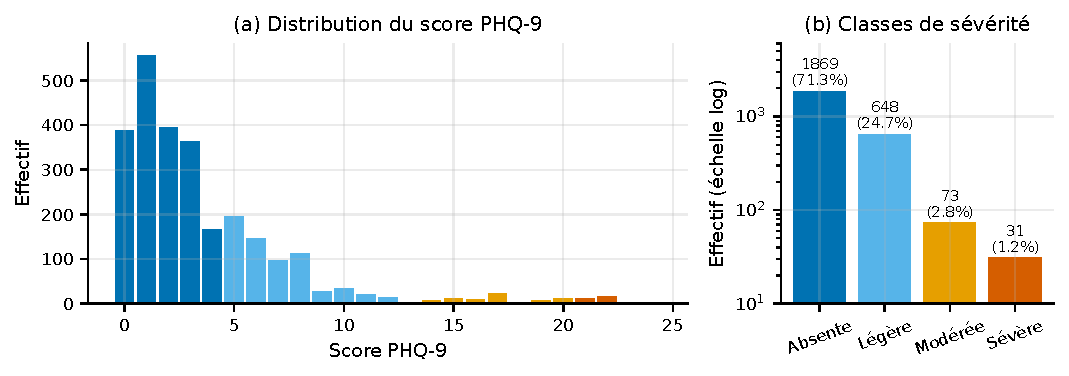
\includegraphics[width=\columnwidth]{../figures/eda_distribution.pdf}
\caption{Distribution du score PHQ-9 et des quatre classes de sévérité.}\label{fig:eda}\end{figure}

\paragraph{Audit de fuite de données.} Un Random Forest par défaut entraîné sur les \emph{trois} biomarqueurs seuls atteint une AUC de 0,94 en validation croisée aléatoire, bien au-delà du 0,84 de l'article avec cinq biomarqueurs et neuf variables, alors que les corrélations sont quasi nulles : ce résultat est suspect. Nous avons donc audité le fichier (figure~\ref{fig:leak}, tableau~\ref{tab:leak}).
\begin{itemize}[leftmargin=*,itemsep=0pt,topsep=2pt]
\item \textbf{Valeurs dupliquées.} 67\,\% (Humanin), 71\,\% (MOTSc) et 85\,\% (P66) des lignes partagent leur valeur avec au moins une autre ligne, ce qui est improbable pour des dosages à deux ou trois décimales. Le plus grand groupe de triplets identiques compte 36 lignes mêlant les deux sexes, les trois génotypes ACE et des âges de 46 à 84 ans : il ne peut s'agir d'une même personne.
\item \textbf{Lien avec la cible.} Les lignes qui partagent un triplet de biomarqueurs ont la même classe de sévérité dans 98,9\,\% des cas, contre 74,0\,\% lorsque les étiquettes sont permutées au hasard.
\item \textbf{Conséquence.} L'AUC de la RF passe de 0,94 (découpage aléatoire) à 0,89 (groupes par triplet), 0,82--0,86 (une ligne par triplet) puis à 0,60 (biomarqueurs seuls) et 0,72 (toutes variables) sur le sous-ensemble de 228 lignes dont \emph{aucune} valeur n'est partagée ; le contrôle par permutation des étiquettes donne bien 0,50 sur le jeu complet.
\end{itemize}
Ces constats sont compatibles avec une imputation par donneurs conditionnée aux classes, telle que décrite dans la méthode de Jelinek \emph{et al.} \cite{jelinek2014} citée par l'article source : les valeurs imputées « encodent » alors la cible. Nous ne pouvons toutefois pas le vérifier sans documentation du jeu de données ; c'est une \emph{hypothèse}. Il est impossible de regrouper les lignes par valeur partagée (une composante connexe unique contient 2\,148 des 2\,621 lignes), d'où deux \textbf{régimes d'analyse} :
\begin{itemize}[leftmargin=*,itemsep=0pt,topsep=2pt]
\item \textbf{complet} (2\,621 lignes) : protocole de l'article ; ses scores doivent être lus comme un plafond \emph{optimiste} ;
\item \textbf{propre} (228 lignes, dont 62 déprimées) : lignes dont les trois valeurs sont uniques dans le fichier, approximation des dosages réellement mesurés. Il ne compte que 7 cas modérés et 3 sévères : seule la tâche binaire y est étudiée. Ce choix peut introduire un biais de sélection.
\end{itemize}

\begin{figure*}[t]\centering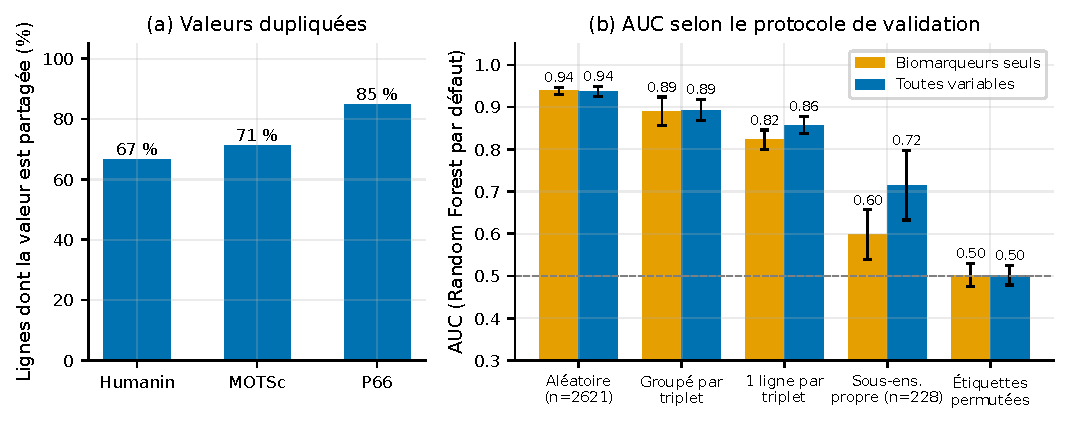
\includegraphics[width=0.82\textwidth]{../figures/leakage_audit.pdf}
\caption{Audit du fichier : (a) part des lignes dont la valeur de biomarqueur est partagée ; (b) AUC d'un Random Forest par défaut selon le protocole de validation (5 répétitions $\times$ 5 plis, barres : écart-type).}\label{fig:leak}\end{figure*}

\begin{table}[t]\centering\caption{AUC du RF par défaut (binaire) selon le protocole de validation (moyenne $\pm$ écart-type sur 25 plis).}\label{tab:leak}
\footnotesize\begin{tabular}{lcc}
\toprule
Protocole & Biomarq. seuls & Toutes var. \\
\midrule
Aléatoire ($n=2621$) & 0,938 $\pm$ 0,009 & 0,937 $\pm$ 0,012 \\
Groupé par triplet & 0,890 $\pm$ 0,034 & 0,893 $\pm$ 0,025 \\
1 ligne/triplet ($n=1571$) & 0,822 $\pm$ 0,023 & 0,858 $\pm$ 0,021 \\
Sous-ens. propre ($n=228$) & 0,598 $\pm$ 0,059 & 0,715 $\pm$ 0,083 \\
\midrule
Permutation ($n=2621$) & 0,502 $\pm$ 0,028 & 0,502 $\pm$ 0,023 \\
Permutation ($n=228$) & 0,518 $\pm$ 0,081 & 0,524 $\pm$ 0,096 \\
\bottomrule
\end{tabular}
\end{table}

\subsection{Reproduction du baseline}
La baseline reprend le protocole de \cite{bader2024} : découpage stratifié 70/30, standardisation, six classifieurs (LR, RF, KNN, SVM, NB, ANN) puis variantes pondérées (WLR, WRF avec les poids de l'éq.~\eqref{eq:weights}) et RF-SMOTE, en classification binaire et à quatre classes, avec deux jeux de variables : biomarqueurs seuls (MDP) et toutes variables (ALL). Les modèles utilisent leurs \textbf{hyperparamètres par défaut} (RF : 100 arbres ; KNN : $k=5$ ; SVM RBF : $C=1$ ; LR : $\ell_2$, $C=1$ ; ANN : une couche cachée de 100 neurones ReLU, 350 itérations, comme indiqué dans l'article), car les grilles de l'annexe de \cite{bader2024} ne figurent pas dans le texte principal. Cette reproduction porte sur le \emph{protocole} et non sur les valeurs : biomarqueurs, effectif (2\,621 contre 830) et nombre de variables (12 contre 14) diffèrent ; seule une comparaison qualitative est possible.

\subsection{Stratégie d'amélioration}
\begin{enumerate}[leftmargin=*,itemsep=0pt,topsep=2pt,label=\textbf{(\Alph*)}]
\item \textbf{Optimisation d'hyperparamètres.} Pour chaque modèle : \texttt{GridSearchCV} (grilles de l'annexe~\ref{app:grids}), \texttt{RandomizedSearchCV} (30 tirages dans des distributions, dont des lois log-uniformes pour $C$, $\gamma$, $\alpha$) et, pour la WRF, une recherche bayésienne TPE (Optuna) sur le même espace et le même budget (30 essais $\times$ 5 plis).
\item \textbf{Pondération et modèle ajouté.} WLR, WRF, RF-SMOTE comme dans l'article, plus WHGB (\emph{gradient boosting} par histogrammes pondéré), pour tester si un autre ensemble d'arbres améliore la WRF.
\item \textbf{Évaluation rigoureuse.} Validation croisée imbriquée (scores appariés avant/après), intervalles de confiance par \emph{bootstrap} sur le test, et régime « propre » de l'audit.
\item \textbf{Inférence statistique} sur les scores appariés (§\ref{sec:proto}).
\end{enumerate}

\subsection{Protocole expérimental}\label{sec:proto}
\paragraph{Séparation des données.} Un découpage 70/30 stratifié (graine 42) isole le jeu de test, utilisé une seule fois par modèle. Toutes les recherches s'exécutent sur les 70\,\% d'entraînement, par validation croisée stratifiée à 5 plis, avec pour critère l'AUC-ROC (macro un-contre-tous à quatre classes). Le meilleur modèle est ré-entraîné sur tout l'entraînement. Parmi les variantes optimisées, la méthode retenue pour les figures est celle dont l'\emph{AUC en validation croisée} est maximale : le test n'intervient jamais dans ce choix.

\paragraph{Répétitions.} Un seul découpage 70/30 produit des estimations très bruitées (le test ne contient que 9 cas sévères dans le jeu complet). Nous ajoutons donc une validation croisée \textbf{imbriquée} : boucle externe stratifiée $5\times2$ (10 scores appariés par modèle), boucle interne = \texttt{RandomizedSearchCV} à 15 candidats et 5 plis. Pour chaque pli externe, le modèle par défaut et le modèle optimisé sont évalués sur le même sous-ensemble de test.

\paragraph{Métriques et tests.} Exactitude, précision, rappel et $F_1$ (pondérés), $F_1$ macro, exactitude équilibrée, AUC-ROC et AUC-PR ; intervalles à 95\,\% par \emph{bootstrap} (1\,000 rééchantillonnages du test). Gain d'optimisation par modèle : $t$ apparié, $t$ corrigé de Nadeau--Bengio ($p_{NB}$) et Wilcoxon ($p_W$, corrigé de Holm sur les dix modèles) ; comparaison des modèles : Friedman et Conover \cite{demsar2006,terpilowski2019}.

\subsection{Implémentation}\label{sec:impl}
Python 3.13.2 ; scikit-learn 1.6.1 \cite{pedregosa2011}, imbalanced-learn 0.14.2 \cite{lemaitre2017}, Optuna 4.3.0 \cite{akiba2019}, SciPy 1.17.1 \cite{virtanen2020}, scikit-posthocs 0.18.0 \cite{terpilowski2019}, statsmodels 0.14.4, pandas 2.2.3 \cite{mckinney2010}, NumPy 2.3.5 \cite{harris2020}, matplotlib 3.10.3 \cite{hunter2007}. Toutes les graines sont fixées à 42 (découpages, modèles, recherches, Optuna). Le standardiseur et SMOTE sont ajustés \emph{à l'intérieur} de chaque pli, via un \texttt{Pipeline} (\texttt{imblearn.pipeline} pour SMOTE), afin d'éviter toute fuite supplémentaire. Le code et les versions exactes sont fournis (\texttt{requirements.txt}, \texttt{README.md}).

\section{Expérimentations et résultats}

\subsection{Environnement de simulation}
Windows~11 Pro, processeur Intel à 12 threads logiques, Python~3.13.2 (versions des bibliothèques au §\ref{sec:impl}). Aucun GPU n'est utilisé : tous les modèles (y compris l'ANN, un \texttt{MLPClassifier}) s'exécutent sur CPU. Les temps sont des durées réelles mesurées avec \texttt{n\_jobs=-1} (12 processus). Sauf mention contraire, les résultats portent sur le \textbf{jeu de test} (30\,\%, 787 lignes dans le régime complet, 69 dans le régime propre).

\subsection{Résultats du baseline}
\begin{table*}[t]\centering\caption{Baseline (hyperparamètres par défaut), régime complet, \emph{toutes variables}, jeu de test. F1$_p$ : $F_1$ pondéré ; F1$_m$ : $F_1$ macro. En gras : meilleure valeur de la colonne.}\label{tab:baseline}
\footnotesize\begin{tabular}{lcccccccccc}
\toprule
& \multicolumn{5}{c}{Binaire} & \multicolumn{5}{c}{4 classes} \\ \cmidrule(lr){2-6}\cmidrule(lr){7-11}
Modèle & Acc. & F1$_p$ & F1$_m$ & AUC & AUC-PR & Acc. & F1$_p$ & F1$_m$ & AUC & AUC-PR \\
\midrule
LR & 0,756 & 0,737 & 0,661 & 0,742 & 0,594 & 0,757 & 0,725 & 0,501 & 0,745 & 0,535 \\
RF & \textbf{0,878} & \textbf{0,875} & \textbf{0,844} & \textbf{0,928} & \textbf{0,876} & \textbf{0,872} & \textbf{0,866} & \textbf{0,706} & \textbf{0,895} & \textbf{0,733} \\
KNN & 0,811 & 0,807 & 0,761 & 0,830 & 0,657 & 0,795 & 0,786 & 0,577 & 0,808 & 0,513 \\
SVM & 0,807 & 0,798 & 0,744 & 0,822 & 0,698 & 0,802 & 0,789 & 0,588 & 0,810 & 0,566 \\
NB & 0,708 & 0,706 & 0,639 & 0,712 & 0,495 & 0,682 & 0,676 & 0,384 & 0,740 & 0,455 \\
ANN & 0,841 & 0,839 & 0,801 & 0,853 & 0,764 & 0,821 & 0,815 & 0,627 & 0,847 & 0,592 \\
\bottomrule
\end{tabular}
\end{table*}

Le tableau~\ref{tab:baseline} reproduit les tableaux~5 et~9 de \cite{bader2024}. Le \textbf{classement qualitatif est celui de l'article} : la RF est la meilleure sur toutes les métriques (AUC 0,928 en binaire, 0,895 à quatre classes), devant l'ANN (0,853 / 0,847), tandis que LR et NB sont les plus faibles (AUC de 0,71 à 0,75). En valeur absolue, nos AUC sont toutefois nettement supérieures à celles de l'article (0,84 et 0,88 pour la RF), ce qui n'est pas attendu avec moins de biomarqueurs.

Le cas des biomarqueurs seuls est révélateur (annexe~\ref{app:full}) : la RF y atteint une AUC de \textbf{0,936} (binaire), \emph{supérieure} à celle obtenue avec toutes les variables (0,928), alors que l'article observe l'inverse (0,81 puis 0,84). Dans le même temps, LR et NB restent au niveau du hasard (0,54 et 0,50), conformément aux corrélations quasi nulles : seul un modèle capable de \og mémoriser \fg{} des combinaisons exactes de valeurs réussit, ce qui est cohérent avec l'audit de la section~4.1. Les matrices de confusion (figure~\ref{fig:cm}) montrent que la classe sévère est correctement reconnue dans 5 cas sur 9 et la classe modérée dans 8 sur 22 pour la RF par défaut.

\begin{figure}[t]\centering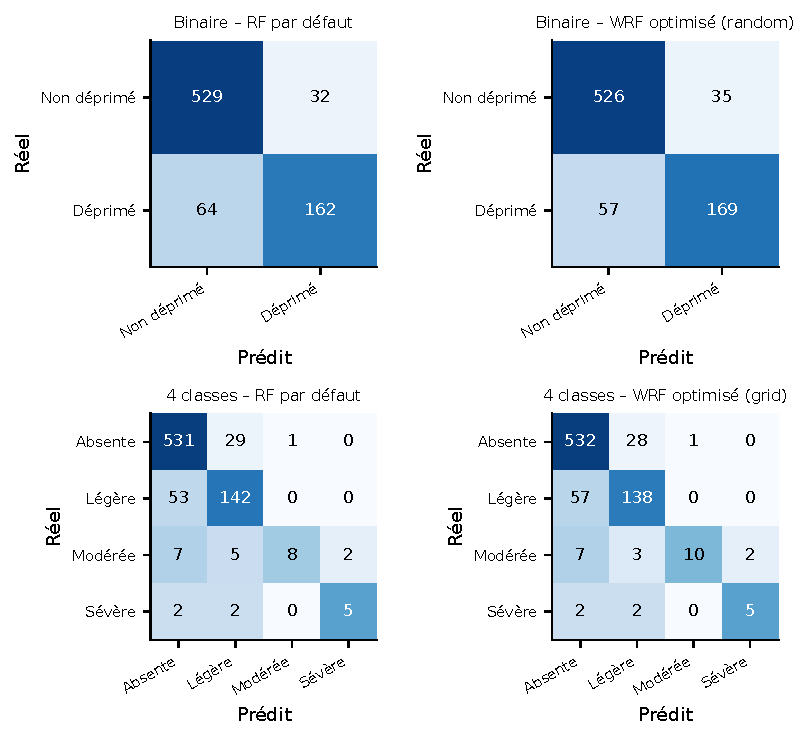
\includegraphics[width=\columnwidth]{../figures/confusion_matrices.pdf}
\caption{Matrices de confusion sur le test (toutes variables, régime complet) : RF par défaut et WRF optimisée, binaire (haut) et quatre classes (bas).}\label{fig:cm}\end{figure}

\subsection{Résultats des améliorations}
\paragraph{(A) Optimisation d'hyperparamètres.} Le tableau~\ref{tab:ba} compare les AUC avant et après optimisation. Dans le \textbf{régime complet}, les ensembles d'arbres sont déjà à leur plafond : la RF passe de 0,928 à 0,926 en binaire, alors que son AUC en validation croisée progresse de 0,935 à 0,942 (tableau~\ref{tab:time}) : le gain observé \emph{en validation} ne se retrouve pas \emph{sur le test}. Les modèles plus sensibles aux réglages gagnent davantage : KNN $+0{,}05$ (binaire) et $+0{,}09$ (quatre classes), SVM $+0{,}02$ à $+0{,}04$. Avec les biomarqueurs seuls, SVM et ANN gagnent jusqu'à $+0{,}14$ et $+0{,}08$ (annexe~\ref{app:full}). Pour la WRF à quatre classes, l'optimisation fait passer l'AUC de 0,903 à 0,927 (grille), 0,919 (aléatoire) et 0,915 (Optuna), valeur proche des 0,91 de l'article, mais les intervalles de confiance se chevauchent largement (tableau~\ref{tab:boot}). Dans le \textbf{régime propre}, l'optimisation n'améliore pas la RF (0,695 $\to$ 0,644 pour la grille) et les écarts restent dans l'incertitude ($\pm 0{,}14$).

\begin{table*}[t]\centering\caption{AUC sur le test avant (Déf.) et après optimisation (Grid, Rand.), toutes variables. En gras : meilleure valeur lorsqu'elle améliore le réglage par défaut.}\label{tab:ba}
\footnotesize\begin{tabular}{lccccccccc}
\toprule
& \multicolumn{3}{c}{Complet, binaire} & \multicolumn{3}{c}{Complet, 4 classes} & \multicolumn{3}{c}{Propre, binaire} \\\cmidrule(lr){2-4}\cmidrule(lr){5-7}\cmidrule(lr){8-10}
Modèle & Déf. & Grid & Rand. & Déf. & Grid & Rand. & Déf. & Grid & Rand. \\
\midrule
LR & 0,742 & 0,742 & \textbf{0,742} & 0,745 & \textbf{0,760} & 0,755 & 0,664 & 0,664 & \textbf{0,673} \\
RF & 0,928 & 0,926 & 0,926 & 0,895 & 0,895 & \textbf{0,906} & 0,695 & 0,644 & 0,682 \\
KNN & 0,830 & 0,877 & \textbf{0,880} & 0,808 & \textbf{0,895} & 0,894 & 0,724 & 0,682 & \textbf{0,726} \\
SVM & 0,822 & \textbf{0,837} & 0,824 & 0,810 & \textbf{0,851} & 0,836 & 0,642 & 0,645 & \textbf{0,646} \\
NB & 0,712 & \textbf{0,713} & 0,712 & 0,740 & \textbf{0,743} & 0,742 & 0,634 & 0,634 & 0,634 \\
ANN & 0,853 & 0,854 & \textbf{0,861} & 0,847 & \textbf{0,854} & 0,851 & 0,627 & \textbf{0,654} & 0,645 \\
\midrule
WLR & 0,739 & \textbf{0,739} & 0,739 & 0,688 & 0,669 & \textbf{0,703} & 0,661 & 0,663 & \textbf{0,665} \\
WRF & 0,923 & \textbf{0,928} & 0,925 & 0,903 & \textbf{0,927} & 0,919 & 0,665 & 0,668 & \textbf{0,705} \\
RF-SMOTE & 0,924 & 0,924 & 0,919 & 0,897 & \textbf{0,911} & 0,891 & 0,727 & 0,706 & 0,724 \\
WHGB & 0,915 & 0,920 & \textbf{0,927} & 0,910 & \textbf{0,916} & 0,915 & 0,683 & \textbf{0,700} & 0,683 \\
\bottomrule
\end{tabular}
\end{table*}

Les hyperparamètres retenus changent de nature selon le régime (figure~\ref{fig:hp}). Dans le régime complet, l'AUC en validation croisée augmente de façon monotone avec la profondeur et diminue quand \texttt{min\_samples\_leaf} croît : l'optimum est l'arbre entièrement développé (\texttt{max\_depth=None}, \texttt{min\_samples\_leaf=1}), avec KNN à pondération par la distance et un SVM à forte capacité ($C\approx 46$, $\gamma\approx 0{,}1$). Dans le régime propre, la surface est quasi plate (0,66--0,72) et favorise des arbres peu profonds (profondeur 3, feuilles de 3) et un SVM très régularisé ($C\approx 0{,}04$) : la recherche y exploite surtout le bruit de la validation croisée.

\begin{figure*}[t]\centering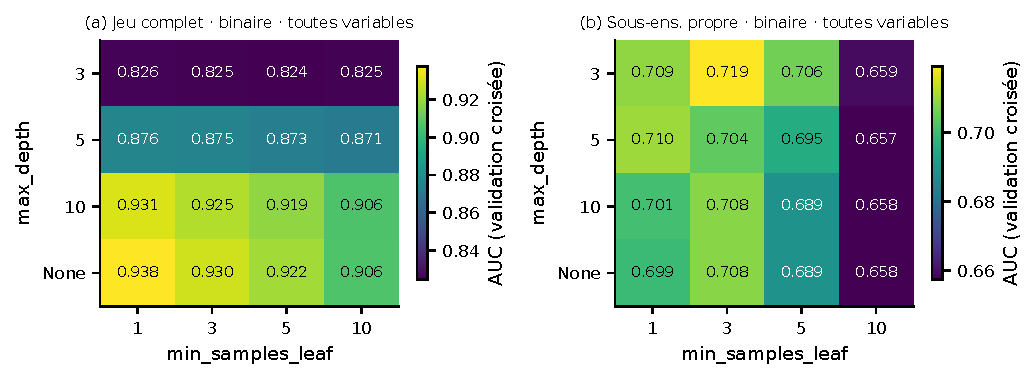
\includegraphics[width=0.78\textwidth]{../figures/hp_sensitivity.pdf}
\caption{Sensibilité de la RF à \texttt{max\_depth} et \texttt{min\_samples\_leaf} (AUC en validation croisée, grille moyennée sur \texttt{n\_estimators} et \texttt{max\_features}).}\label{fig:hp}\end{figure*}

\paragraph{(B) Pondération, SMOTE et modèle ajouté.} Le tableau~\ref{tab:weighted} confirme l'ordre de l'article à quatre classes (WRF $>$ RF-SMOTE $>$ WLR) : AUC de 0,903, 0,897 et 0,688 par défaut. La WLR s'effondre (exactitude 0,48, $F_{1,m}$ 0,33) : avec des poids atteignant $W\approx 21$ pour la classe sévère, un modèle linéaire sur-prédit les classes rares. La WRF améliore peu l'exactitude équilibrée de la RF (0,644 par défaut, 0,667 optimisée, contre 0,648) ; en binaire elle n'apporte rien (0,923 contre 0,928). Le modèle ajouté, WHGB, est compétitif : meilleur $F_{1,m}$ (0,738) et meilleure exactitude équilibrée (0,693) à quatre classes par défaut.

\begin{table}[t]\centering\caption{Modèles pondérés avant/après optimisation (méthode retenue d'après l'AUC en validation croisée), régime complet, \emph{quatre classes}, toutes variables ; Acc.$_{éq}$ : exactitude équilibrée.}\label{tab:weighted}
\scriptsize\begin{tabular}{lcccccc}
\toprule
\multicolumn{7}{l}{\textit{Complet, 4 classes, toutes var.}} \\ \midrule
Modèle & Acc. & F1$_p$ & F1$_m$ & Acc.$_{éq}$ & AUC & AUC-PR \\
\midrule
RF & 0,872 & 0,866 & 0,706 & 0,648 & 0,895 & 0,733 \\
RF (grid) & 0,869 & 0,865 & 0,726 & 0,669 & 0,895 & 0,743 \\
WLR & 0,478 & 0,562 & 0,329 & 0,490 & 0,688 & 0,371 \\
WLR (random) & 0,546 & 0,612 & 0,327 & 0,467 & 0,703 & 0,487 \\
WRF & 0,869 & 0,863 & 0,717 & 0,644 & 0,903 & 0,746 \\
WRF (grid) & 0,870 & 0,865 & 0,726 & 0,667 & 0,927 & 0,748 \\
RF-SMOTE & 0,844 & 0,843 & 0,685 & 0,661 & 0,897 & 0,723 \\
RF-SMOTE (grid) & 0,849 & 0,848 & 0,694 & 0,665 & 0,911 & 0,711 \\
WHGB & 0,875 & 0,874 & 0,738 & 0,693 & 0,910 & 0,756 \\
WHGB (random) & 0,874 & 0,873 & 0,720 & 0,690 & 0,915 & 0,725 \\
WRF (optuna) & 0,861 & 0,857 & 0,736 & 0,665 & 0,915 & 0,740 \\
\bottomrule
\end{tabular}
\end{table}

\paragraph{Courbes ROC et d'apprentissage.} Les courbes ROC des RF, WRF et RF-SMOTE se superposent presque dans le régime complet (figure~\ref{fig:roc}a), alors qu'elles sont très irrégulières et mêlées dans le régime propre (figure~\ref{fig:roc}b), où le test ne compte que 19 cas positifs. À quatre classes, la classe modérée est la moins bien séparée (figure~\ref{fig:roc}c). Les courbes d'apprentissage (figure~\ref{fig:lc}) montrent une AUC d'entraînement égale à 1 dans le régime complet et une AUC de validation qui progresse encore à pleine taille (0,92 à 0,94) : l'ajout de données serait plus utile que l'optimisation. Dans le régime propre, la validation plafonne vers 0,66 avec un écart-type large.

\begin{figure*}[t]\centering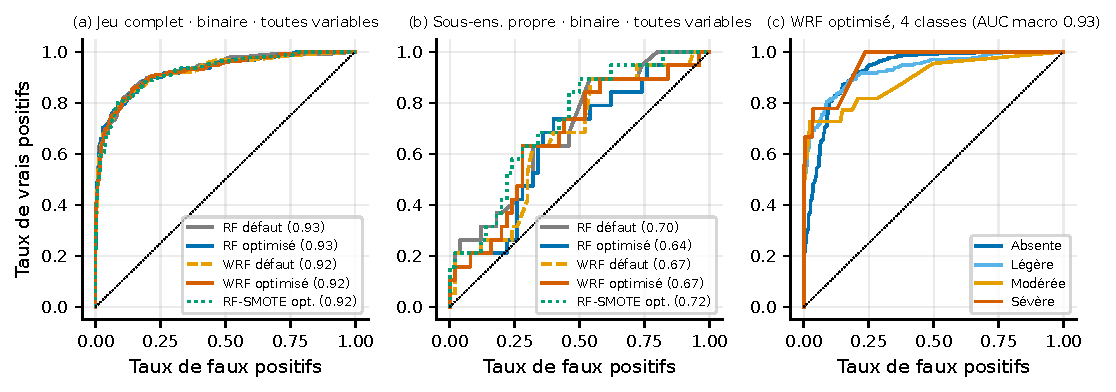
\includegraphics[width=0.92\textwidth]{../figures/roc_curves.pdf}
\caption{Courbes ROC sur le test : binaire, régime complet (a) et propre (b), toutes variables (AUC entre parenthèses) ; WRF optimisée à quatre classes, un-contre-tous (c).}\label{fig:roc}\end{figure*}

\begin{figure*}[t]\centering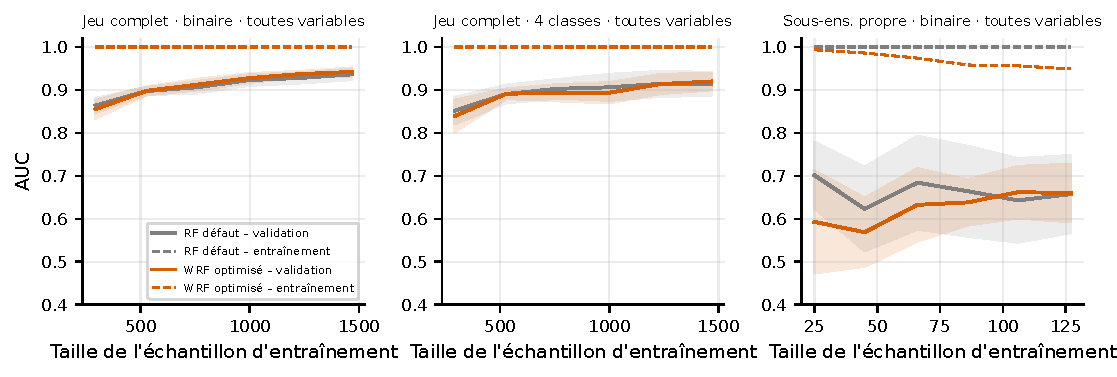
\includegraphics[width=0.92\textwidth]{../figures/learning_curves.pdf}
\caption{Courbes d'apprentissage (validation croisée à 5 plis sur l'entraînement ; bandes : $\pm1$ écart-type).}\label{fig:lc}\end{figure*}

\subsection{Comparaison baseline et améliorations}
\paragraph{Coût de calcul.} Le tableau~\ref{tab:time} met en regard le nombre d'ajustements, le temps et l'AUC en validation croisée. Pour la RF, la recherche aléatoire atteint la même qualité que la grille (0,942 contre 0,941) avec 150 au lieu de 320 ajustements ; Optuna (0,942 pour la WRF, 150 ajustements, 33\,s) fait aussi bien. Pour LR, NB et KNN, le coût est négligeable ; pour l'ANN, 41 à 55\,s de calcul n'apportent aucun gain sur le test dans le régime complet (0,853 $\to$ 0,854 / 0,861). À budget équivalent, aucune des trois stratégies ne domine nettement : le gain tient davantage au \emph{choix du modèle} qu'à celui de la méthode de recherche.

\begin{table}[t]\centering\caption{Coût et score de validation (régime complet, binaire, toutes variables) : nombre d'ajustements, temps réel (s) et AUC en validation croisée.}\label{tab:time}
\scriptsize\begin{tabular}{lcrrrrccc}
\toprule
Modèle & Déf. & \multicolumn{2}{c}{Grid} & \multicolumn{2}{c}{Random} & \multicolumn{3}{c}{AUC-VC} \\\cmidrule(lr){3-4}\cmidrule(lr){5-6}\cmidrule(lr){7-9}
 & (s) & fits & s & fits & s & Déf. & Grid & Rand. \\
\midrule
LR & 0,01 & 50 & 0 & 150 & 1 & 0,762 & 0,762 & 0,762 \\
RF & 0,39 & 320 & 32 & 150 & 25 & 0,935 & 0,941 & 0,942 \\
KNN & 0,01 & 160 & 2 & 150 & 2 & 0,834 & 0,888 & 0,888 \\
SVM & 0,70 & 80 & 9 & 150 & 17 & 0,837 & 0,852 & 0,846 \\
NB & 0,00 & 45 & 0 & 150 & 0 & 0,723 & 0,725 & 0,724 \\
ANN & 1,86 & 160 & 41 & 150 & 55 & 0,883 & 0,883 & 0,883 \\
WLR & 0,01 & 50 & 0 & 150 & 0 & 0,763 & 0,763 & 0,763 \\
WRF & 0,30 & 320 & 31 & 150 & 27 & 0,936 & 0,942 & 0,943 \\
RF-SMOTE & 0,38 & 360 & 45 & 150 & 26 & 0,934 & 0,939 & 0,936 \\
WHGB & 1,29 & 360 & 15 & 150 & 12 & 0,931 & 0,935 & 0,934 \\
\bottomrule
\end{tabular}

\smallskip\noindent\footnotesize Optuna (TPE, WRF) : 150 fits, 33\,s.
\end{table}

\paragraph{Incertitude.} Le tableau~\ref{tab:boot} donne les intervalles de confiance à 95\,\% de l'AUC de test. Dans le régime complet, ils mesurent $\pm 0{,}02$ en binaire et $\pm 0{,}05$ à quatre classes ; dans le régime propre, $\pm 0{,}14$. Pour chaque cadre, les intervalles des quatre variantes se chevauchent ; la plus forte hausse (WRF à quatre classes, toutes variables, $+0{,}024$ sur la WRF par défaut) ne s'en détache donc pas à l'échelle d'un seul découpage, d'où la validation imbriquée ci-dessous.

\begin{table*}[t]\centering\caption{AUC de test et intervalle de confiance \emph{bootstrap} à 95\,\% (1\,000 rééchantillonnages) ; variante optimisée choisie d'après l'AUC en validation croisée.}\label{tab:boot}
\footnotesize\begin{tabular}{lcccc}
\toprule
Cadre & RF défaut & RF optimisé & WRF défaut & WRF optimisé \\
\midrule
Complet, binaire, biomarq. & 0,936 [0,917 ; 0,954] & 0,936 [0,918 ; 0,955] & 0,932 [0,912 ; 0,951] & 0,935 [0,916 ; 0,953] \\
Complet, binaire, toutes var. & 0,928 [0,906 ; 0,948] & 0,926 [0,904 ; 0,946] & 0,923 [0,901 ; 0,945] & 0,925 [0,903 ; 0,945] \\
Complet, 4 classes, biomarq. & 0,898 [0,845 ; 0,951] & 0,893 [0,839 ; 0,949] & 0,896 [0,842 ; 0,947] & 0,896 [0,843 ; 0,950] \\
Complet, 4 classes, toutes var. & 0,895 [0,842 ; 0,943] & 0,895 [0,836 ; 0,946] & 0,903 [0,851 ; 0,950] & 0,927 [0,898 ; 0,954] \\
Propre, binaire, biomarq. & 0,676 [0,530 ; 0,816] & 0,621 [0,477 ; 0,767] & 0,649 [0,503 ; 0,788] & 0,611 [0,464 ; 0,762] \\
Propre, binaire, toutes var. & 0,695 [0,558 ; 0,832] & 0,644 [0,488 ; 0,793] & 0,665 [0,520 ; 0,806] & 0,668 [0,523 ; 0,814] \\
\bottomrule
\end{tabular}
\end{table*}

\subsection{Analyse statistique}
Les tests s'appuient sur les 10 scores appariés (AUC) de la validation croisée imbriquée. \textbf{Gain de l'optimisation.} Le tableau~\ref{tab:gain} donne, pour chaque modèle, l'AUC par défaut (AUC$_0$), le gain moyen $\Delta$ = AUC(optimisé) $-$ AUC(défaut), la valeur $p_W$ du test de Wilcoxon (corrigée de Holm sur les dix modèles) et la valeur $p_{NB}$ du test $t$ corrigé de Nadeau--Bengio ; la figure~\ref{fig:nested} en montre la dispersion sur les six cadres.

\begin{table*}[t]\centering\caption{Gain d'AUC dû à l'optimisation (recherche aléatoire interne) en validation croisée imbriquée $5\times2$, toutes variables : AUC$_0$ par défaut, gain moyen $\Delta$, $p_W$ (Wilcoxon, Holm) et $p_{NB}$ ($t$ corrigé).}\label{tab:gain}
\scriptsize\setlength{\tabcolsep}{2.6pt}\begin{tabular}{lcccccccccccc}
\toprule
& \multicolumn{4}{c}{Complet, binaire} & \multicolumn{4}{c}{Complet, 4 classes} & \multicolumn{4}{c}{Propre, binaire} \\\cmidrule(lr){2-5}\cmidrule(lr){6-9}\cmidrule(lr){10-13}
Modèle & AUC$_0$ & $\Delta$ & $p_W$ & $p_{NB}$ & AUC$_0$ & $\Delta$ & $p_W$ & $p_{NB}$ & AUC$_0$ & $\Delta$ & $p_W$ & $p_{NB}$ \\
\midrule
LR & 0,753 & $-$0,000 & 1,000 & 0,712 & 0,773 & +0,004 & 1,000 & 0,553 & 0,722 & $-$0,005 & 1,000 & 0,570 \\
RF & 0,939 & $-$0,007 & 0,047 & 0,052 & 0,926 & +0,008 & 0,451 & 0,273 & 0,716 & $-$0,029 & 0,039 & 0,054 \\
KNN & 0,849 & +0,041 & 0,020 & 0,003 & 0,823 & +0,063 & 0,020 & 0,003 & 0,650 & +0,032 & 0,781 & 0,349 \\
SVM & 0,840 & +0,009 & 0,322 & 0,271 & 0,852 & $-$0,000 & 1,000 & 0,987 & 0,688 & $-$0,012 & 1,000 & 0,680 \\
NB & 0,720 & +0,000 & 0,020 & 0,052 & 0,753 & +0,001 & 0,246 & 0,190 & 0,696 & $-$0,001 & 1,000 & 0,664 \\
ANN & 0,885 & $-$0,006 & 0,293 & 0,317 & 0,868 & +0,009 & 0,297 & 0,252 & 0,665 & +0,021 & 0,246 & 0,107 \\
\midrule
WLR & 0,753 & $-$0,000 & 1,000 & 0,594 & 0,683 & +0,006 & 1,000 & 0,881 & 0,726 & $-$0,001 & 1,000 & 0,939 \\
WRF & 0,938 & $-$0,005 & 0,336 & 0,290 & 0,919 & +0,009 & 0,785 & 0,379 & 0,701 & $-$0,014 & 0,961 & 0,514 \\
RF-SMOTE & 0,937 & $-$0,004 & 0,137 & 0,175 & 0,919 & $-$0,001 & 1,000 & 0,926 & 0,705 & $-$0,016 & 1,000 & 0,643 \\
WHGB & 0,928 & +0,002 & 1,000 & 0,754 & 0,928 & $-$0,002 & 0,785 & 0,614 & 0,680 & +0,017 & 0,916 & 0,575 \\
\bottomrule
\end{tabular}
\end{table*}

Dans le régime complet, l'optimisation ne procure un gain significatif qu'à \textbf{KNN} ($+0{,}041$ en binaire, $+0{,}063$ à quatre classes ; $p_W=0{,}020$, valeur minimale atteignable avec 10 paires après correction de Holm ; $p_{NB}=0{,}003$). Les autres modèles ne montrent aucun gain significatif et la RF \emph{perd} $0{,}007$ en binaire ($p_W=0{,}047$) : avec 15 candidats, la sélection interne est bruitée alors que le réglage par défaut est déjà presque optimal. NB affiche un écart « significatif » mais négligeable ($+0{,}0005$). Avec les biomarqueurs seuls, KNN ($+0{,}048$), SVM ($+0{,}115$) et ANN ($+0{,}056$) gagnent significativement en binaire ($p_W=0{,}020$), et de même à quatre classes ($+0{,}035$, $+0{,}068$, $+0{,}054$). Dans le \textbf{régime propre}, aucun gain n'est significatif et la RF perd $0{,}029$ ($p_W=0{,}039$).

\begin{figure*}[t]\centering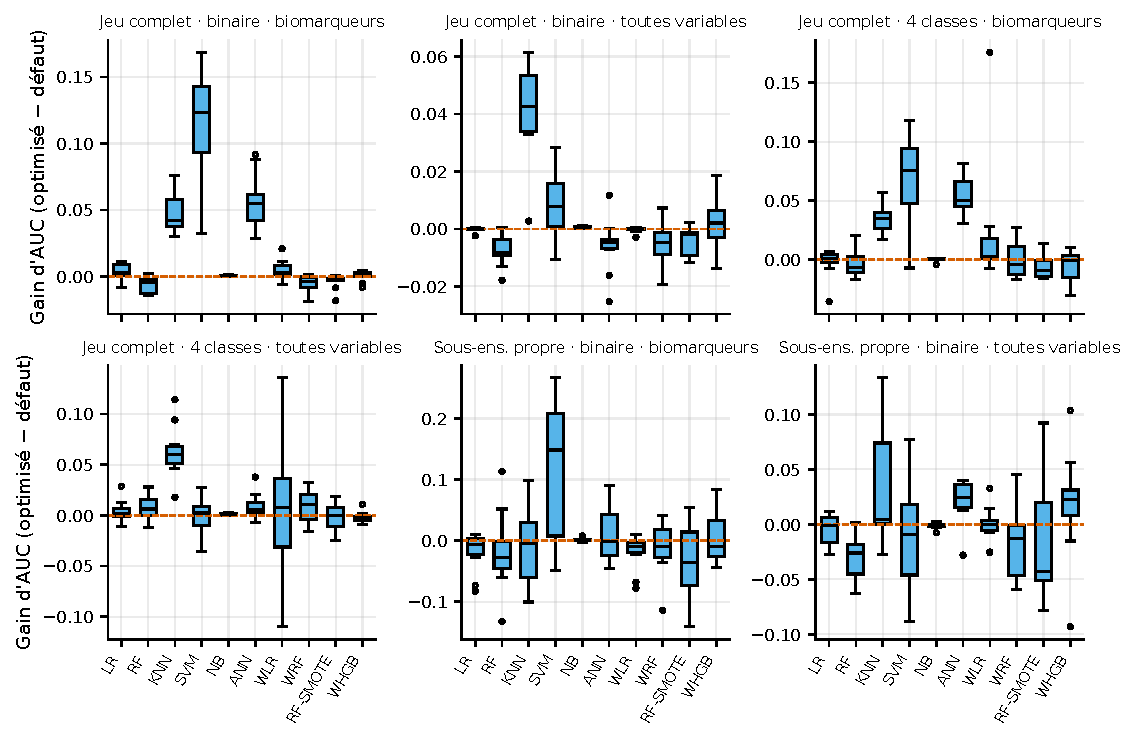
\includegraphics[width=0.78\textwidth]{../figures/nested_gain.pdf}
\caption{Gain d'AUC (optimisé $-$ défaut) sur les 10 plis externes de la validation croisée imbriquée, par modèle et par cadre.}\label{fig:nested}\end{figure*}

\textbf{Comparaison des modèles.} Dans le régime complet, le test de Friedman rejette l'égalité des six classifieurs de base ($\chi^2\approx 46$--$49$, $p<10^{-3}$) et la RF est significativement supérieure à chacun des autres (Conover--Holm, $p<10^{-3}$ ; seule exception, RF--KNN optimisé sur les biomarqueurs seuls : $p=0{,}047$), ce qui \textbf{reproduit} le résultat de l'article (tableau~\ref{tab:friedman}). Dans le régime propre, le test n'est significatif que par défaut ($p_F=0{,}015$, seule la paire RF--KNN ressort) et plus du tout après optimisation ($p_F=0{,}63$) : les six classifieurs y sont indiscernables.

\begin{table*}[t]\centering\caption{Tests de Friedman et post-hoc de Conover (valeurs $p$ corrigées de Holm) sur les 10 plis externes : à gauche les six classifieurs de base (RF contre chaque autre modèle), à droite les modèles pondérés (WRF contre WLR et RF-SMOTE).}\label{tab:friedman}
\scriptsize\setlength{\tabcolsep}{2.4pt}\begin{tabular}{llccccccccccc}
\toprule
& & \multicolumn{7}{c}{Six classifieurs de base (RF contre\,\dots)} & \multicolumn{4}{c}{Modèles pondérés (WRF contre\,\dots)} \\\cmidrule(lr){3-9}\cmidrule(lr){10-13}
Cadre & Variante & $\chi^2$ & $p_F$ & LR & KNN & SVM & NB & ANN & $\chi^2$ & $p_F$ & WLR & RF-SMOTE \\
\midrule
Complet, binaire, toutes var. & défaut & 48,8 & $<\!10^{-3}$ & $<\!10^{-3}$ & $<\!10^{-3}$ & $<\!10^{-3}$ & $<\!10^{-3}$ & $<\!10^{-3}$ & 15,8 & $<\!10^{-3}$ & $<\!10^{-3}$ & 0,081 \\
 & optimisé & 47,3 & $<\!10^{-3}$ & $<\!10^{-3}$ & $<\!10^{-3}$ & $<\!10^{-3}$ & $<\!10^{-3}$ & $<\!10^{-3}$ & 15,0 & $<\!10^{-3}$ & $<\!10^{-3}$ & 1,000 \\
\midrule
Complet, 4 classes, toutes var. & défaut & 48,0 & $<\!10^{-3}$ & $<\!10^{-3}$ & $<\!10^{-3}$ & $<\!10^{-3}$ & $<\!10^{-3}$ & $<\!10^{-3}$ & 15,8 & $<\!10^{-3}$ & $<\!10^{-3}$ & 0,081 \\
 & optimisé & 47,4 & $<\!10^{-3}$ & $<\!10^{-3}$ & $<\!10^{-3}$ & $<\!10^{-3}$ & $<\!10^{-3}$ & $<\!10^{-3}$ & 15,8 & $<\!10^{-3}$ & $<\!10^{-3}$ & 0,081 \\
\midrule
Complet, binaire, biomarq. & défaut & 48,6 & $<\!10^{-3}$ & $<\!10^{-3}$ & $<\!10^{-3}$ & $<\!10^{-3}$ & $<\!10^{-3}$ & $<\!10^{-3}$ & 15,0 & $<\!10^{-3}$ & $<\!10^{-3}$ & 1,000 \\
 & optimisé & 46,3 & $<\!10^{-3}$ & $<\!10^{-3}$ & 0,047 & $<\!10^{-3}$ & $<\!10^{-3}$ & $<\!10^{-3}$ & 15,2 & $<\!10^{-3}$ & $<\!10^{-3}$ & 0,398 \\
\midrule
Propre, binaire, toutes var. & défaut & 14,1 & 0,015 & 1,000 & 0,024 & 1,000 & 1,000 & 0,059 & 4,2 & 0,122 & 0,137 & 0,339 \\
 & optimisé & 3,4 & 0,631 & 1,000 & 1,000 & 1,000 & 1,000 & 1,000 & 2,6 & 0,273 & 0,541 & 0,655 \\
\bottomrule
\end{tabular}
\end{table*}

Parmi les modèles pondérés (partie droite du tableau~\ref{tab:friedman}), la WRF est significativement meilleure que la WLR dans le régime complet ($p<10^{-3}$), mais pas que RF-SMOTE au seuil de 5\,\% ($p=0{,}081$ à quatre classes, par défaut comme optimisée) : la supériorité de la WRF sur RF-SMOTE n'apparaît qu'au seuil de 10\,\%, comme dans l'article (qui retient $\alpha=0{,}1$ pour toutes les variables).

\textbf{Jeux de variables.} Pour la WRF optimisée, ajouter les variables cliniques n'améliore pas l'AUC en binaire dans le régime complet ($+0{,}002$, $p_W=0{,}70$) : les seuls biomarqueurs suffisent, ce qui contredit l'article. L'ajout aide à quatre classes ($+0{,}025$, $p_W=0{,}020$, $p_{NB}=0{,}13$) et nettement dans le régime propre ($+0{,}090$, $p_W=0{,}004$, $p_{NB}=0{,}038$) : sans doublons, l'essentiel du signal vient des variables cliniques.

\subsection{Discussion}
\paragraph{Qui gagne à l'optimisation ?} Les modèles dont les réglages par défaut sont mal adaptés (KNN, SVM, ANN) gagnent de $+0{,}04$ à $+0{,}12$ d'AUC dans le régime complet ; les ensembles d'arbres, déjà proches de leur plafond, ne gagnent rien (RF et WRF : $-0{,}007$ à $+0{,}009$, non significatif ou négatif) et leur AUC varie peu autour des bons réglages (figure~\ref{fig:hp}). Grille, recherche aléatoire et TPE donnent des scores équivalents à budget comparable (tableau~\ref{tab:time}) : la valeur ajoutée dépend du \emph{modèle} plus que de la \emph{stratégie} de recherche. Dans le régime propre, les écarts entre configurations (0,66--0,72) sont du même ordre que l'écart-type entre plis (0,06--0,08) : la sélection suit surtout le bruit, d'où le gain négatif de la RF.

\paragraph{Une optimisation qui apprend la fuite ?} Dans le régime complet, les gains vont aux modèles capables d'\emph{interpoler} des valeurs dupliquées, et les réglages choisis sont de capacité maximale (arbres entièrement développés, KNN pondéré par la distance, SVM à $C\approx 46$). Cinq indices concordent avec l'hypothèse de fuite : (i) la RF atteint 0,94 avec trois biomarqueurs presque non corrélés à la cible ($|r|\leq 0{,}06$), alors que LR et NB restent à 0,5 ; (ii) les biomarqueurs seuls égalent les toutes variables ; (iii) l'optimum de profondeur est « le plus profond » dans le régime complet, mais s'inverse dans le régime propre (figure~\ref{fig:hp}) ; (iv) l'importance par permutation (figure~\ref{fig:perm}) place P66, MOTS-c et Humanin en tête dans le régime complet, puis s'annule pour eux dans le régime propre où le diabète domine ; (v) l'AUC tombe de 0,94 à 0,60 (biomarqueurs seuls) sans lignes à valeurs partagées. La conclusion de l'article selon laquelle les biomarqueurs sont les variables les plus importantes n'est donc \emph{pas robuste} sur ce fichier. Nous ne savons pas si les données de l'article ont le même défaut ; sa méthode d'imputation par classes en fait toutefois un point à vérifier.

\begin{figure*}[t]\centering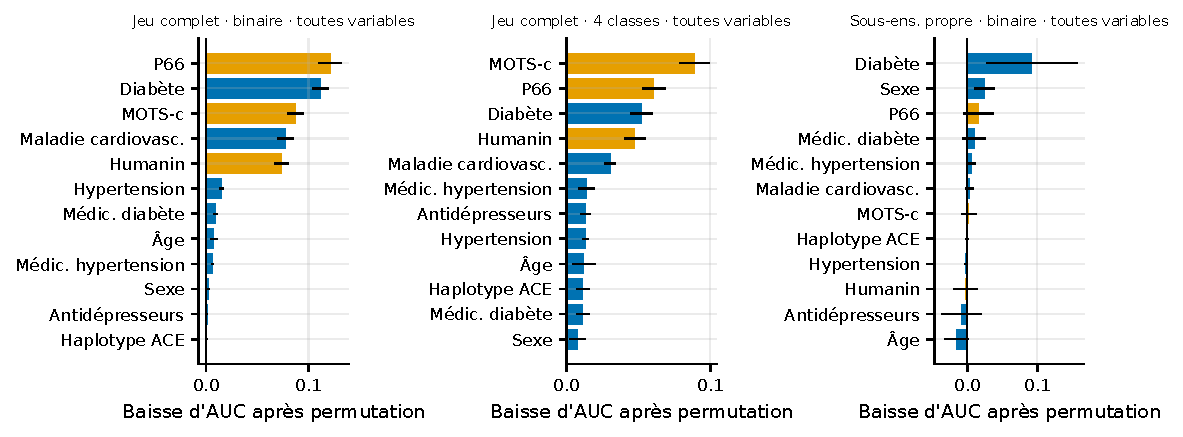
\includegraphics[width=0.92\textwidth]{../figures/permutation_importance.pdf}
\caption{Importance par permutation pour la WRF optimisée (30 permutations, jeu de test) ; orange : biomarqueurs.}\label{fig:perm}\end{figure*}

\paragraph{Limites et cas d'échec.} Le régime propre ne compte que 228 lignes (62 déprimées) : la puissance statistique est faible, la tâche à quatre classes y est impossible (3 cas sévères) et le choix du sous-ensemble peut introduire un biais de sélection. La WLR s'effondre à quatre classes (poids jusqu'à 21, exactitude 0,48) ; NB et LR sont inopérants sur les biomarqueurs seuls ; le SVM par défaut est sous le hasard sur les biomarqueurs du régime propre (0,44) et l'optimisation le ramène au hasard (0,55, non significatif). L'apport de la pondération reste modeste, y compris pour les métriques sensibles au déséquilibre (exactitude équilibrée de la WRF : 0,644 à 0,667 contre 0,648 pour la RF).

\section{Conclusion et perspectives}

\subsection{Rappel des objectifs}
Nous voulions reproduire le protocole de Bader \emph{et al.} \cite{bader2024} sur le jeu de données fourni, y mettre en place un pipeline complet d'optimisation d'hyperparamètres (\texttt{GridSearchCV}, \texttt{RandomizedSearchCV}, TPE) sous validation croisée stratifiée, et comparer les performances avant et après optimisation.

\subsection{Synthèse des résultats}
\textbf{Reproduit :} le protocole (découpage 70/30, validation croisée à 5 plis, six classifieurs, pondération, SMOTE, tests de Friedman et de Conover), le classement qualitatif (RF meilleure, LR et NB les plus faibles, WRF $\gg$ WLR, WRF $\gtrsim$ RF-SMOTE au seuil de 10\,\%). \textbf{Amélioré :} un pipeline reproductible comparant grille, recherche aléatoire et bayésienne à budget équivalent, avec temps de calcul, validation imbriquée et tests appariés. L'optimisation ne profite \emph{significativement} qu'à KNN, SVM et ANN (de $+0{,}04$ à $+0{,}12$ d'AUC) ; elle est sans effet sur RF et WRF (AUC $\approx 0{,}93$, test) et ne rend pas la WRF significativement meilleure que RF-SMOTE au seuil de 5\,\%. \textbf{Découvert :} le fichier fournit des valeurs de biomarqueurs dupliquées entre lignes et presque parfaitement alignées sur la classe de sévérité ; sans ces lignes, l'AUC chute à 0,60 (biomarqueurs) et 0,72 (toutes variables) et plus aucune optimisation ne profite aux modèles.

\subsection{Limites}
Un seul jeu de données, dont l'origine des valeurs dupliquées n'est pas documentée (hypothèse d'imputation non vérifiée) ; un sous-ensemble « propre » de 228 lignes, trop petit pour la tâche à quatre classes et pour des conclusions fines ; des biomarqueurs différents de ceux de l'article, donc une reproduction de protocole et non de valeurs ; pas de validation externe ; un budget de recherche limité (30 tirages, 15 en validation imbriquée).

\subsection{Perspectives}
(i) Obtenir les données non imputées et un identifiant patient pour une validation \emph{groupée par patient} et un filtrage sur la dernière visite, comme dans l'article ; (ii) imputer à l'intérieur de chaque pli et sans utiliser la cible ; (iii) tester SMOTE-NC, le réglage du seuil de décision et l'étalonnage des probabilités pour la classe sévère ; (iv) appliquer le pipeline à d'autres jeux (par ex.\ données de prêt bancaire, comme le suggère le sujet) ; (v) ajouter des méthodes d'explicabilité. Tant que la question de la fuite n'est pas résolue, ce modèle ne doit pas être déployé comme outil d'aide à la décision clinique.


\begin{thebibliography}{99}\footnotesize
\setlength{\itemsep}{0pt}\setlength{\parskip}{0pt}

\bibitem{bader2024} M.~Bader, M.~Abdelwanis, M.~Maalouf et H.~F.~Jelinek, « Detecting depression severity using weighted random forest and oxidative stress biomarkers », \emph{Sci. Rep.}, vol.~14, art.~16328, 2024, doi:10.1038/s41598-024-67251-y.

\bibitem{breiman2001} L.~Breiman, « Random forests », \emph{Mach. Learn.}, vol.~45, no~1, pp.~5--32, 2001.

\bibitem{chen2004} C.~Chen, A.~Liaw et L.~Breiman, « Using random forest to learn imbalanced data », Dept. of Statistics, Univ. of California, Berkeley, Tech. Rep.~666, 2004.

\bibitem{maalouf2014} M.~Maalouf et M.~Siddiqi, « Weighted logistic regression for large-scale imbalanced and rare events data », \emph{Knowl.-Based Syst.}, vol.~59, pp.~142--148, 2014.

\bibitem{zhang2016} C.~Zhang, Y.~Li, Z.~Yu et F.~Tian, « A weighted random forest approach to improve predictive performance for power system transient stability assessment », in \emph{Proc. IEEE PES APPEEC}, 2016, pp.~1259--1263.

\bibitem{chawla2002} N.~V.~Chawla, K.~W.~Bowyer, L.~O.~Hall et W.~P.~Kegelmeyer, « SMOTE: Synthetic minority over-sampling technique », \emph{J. Artif. Intell. Res.}, vol.~16, pp.~321--357, 2002.

\bibitem{bergstra2012} J.~Bergstra et Y.~Bengio, « Random search for hyper-parameter optimization », \emph{J. Mach. Learn. Res.}, vol.~13, pp.~281--305, 2012.

\bibitem{bergstra2011} J.~Bergstra, R.~Bardenet, Y.~Bengio et B.~K\'egl, « Algorithms for hyper-parameter optimization », in \emph{Adv. Neural Inf. Process. Syst. (NIPS)}, vol.~24, 2011, pp.~2546--2554.

\bibitem{akiba2019} T.~Akiba, S.~Sano, T.~Yanase, T.~Ohta et M.~Koyama, « Optuna: A next-generation hyperparameter optimization framework », in \emph{Proc. ACM SIGKDD}, 2019, pp.~2623--2631.

\bibitem{kohavi1995} R.~Kohavi, « A study of cross-validation and bootstrap for accuracy estimation and model selection », in \emph{Proc. IJCAI}, 1995, pp.~1137--1143.

\bibitem{cawley2010} G.~C.~Cawley et N.~L.~C.~Talbot, « On over-fitting in model selection and subsequent selection bias in performance evaluation », \emph{J. Mach. Learn. Res.}, vol.~11, pp.~2079--2107, 2010.

\bibitem{kaufman2012} S.~Kaufman, S.~Rosset, C.~Perlich et O.~Stitelman, « Leakage in data mining: Formulation, detection, and avoidance », \emph{ACM Trans. Knowl. Discov. Data}, vol.~6, no~4, art.~15, 2012.

\bibitem{nadeau2003} C.~Nadeau et Y.~Bengio, « Inference for the generalization error », \emph{Mach. Learn.}, vol.~52, no~3, pp.~239--281, 2003.

\bibitem{dietterich1998} T.~G.~Dietterich, « Approximate statistical tests for comparing supervised classification learning algorithms », \emph{Neural Comput.}, vol.~10, no~7, pp.~1895--1923, 1998.

\bibitem{demsar2006} J.~Dem\v{s}ar, « Statistical comparisons of classifiers over multiple data sets », \emph{J. Mach. Learn. Res.}, vol.~7, pp.~1--30, 2006.

\bibitem{friedman1937} M.~Friedman, « The use of ranks to avoid the assumption of normality implicit in the analysis of variance », \emph{J. Am. Stat. Assoc.}, vol.~32, no~200, pp.~675--701, 1937.

\bibitem{conover1999} W.~J.~Conover, \emph{Practical Nonparametric Statistics}, 3rd ed. New York: Wiley, 1999.

\bibitem{pereira2015} D.~G.~Pereira, A.~Afonso et F.~M.~Medeiros, « Overview of Friedman's test and post-hoc analysis », \emph{Commun. Stat. Simul. Comput.}, vol.~44, no~10, pp.~2636--2653, 2015.

\bibitem{wilcoxon1945} F.~Wilcoxon, « Individual comparisons by ranking methods », \emph{Biometrics Bull.}, vol.~1, no~6, pp.~80--83, 1945.

\bibitem{kroenke2001} K.~Kroenke, R.~L.~Spitzer et J.~B.~W.~Williams, « The PHQ-9: Validity of a brief depression severity measure », \emph{J. Gen. Intern. Med.}, vol.~16, no~9, pp.~606--613, 2001.

\bibitem{altmann2010} A.~Altmann, L.~Tolo\c{s}i, O.~Sander et T.~Lengauer, « Permutation importance: a corrected feature importance measure », \emph{Bioinformatics}, vol.~26, no~10, pp.~1340--1347, 2010.

\bibitem{saito2015} T.~Saito et M.~Rehmsmeier, « The precision-recall plot is more informative than the ROC plot when evaluating binary classifiers on imbalanced datasets », \emph{PLoS ONE}, vol.~10, no~3, e0118432, 2015.

\bibitem{fawcett2006} T.~Fawcett, « An introduction to ROC analysis », \emph{Pattern Recognit. Lett.}, vol.~27, no~8, pp.~861--874, 2006.

\bibitem{hastie2009} T.~Hastie, R.~Tibshirani et J.~Friedman, \emph{The Elements of Statistical Learning}, 2nd ed. New York: Springer, 2009.

\bibitem{sau2017} A.~Sau et I.~Bhakta, « Predicting anxiety and depression in elderly patients using machine learning technology », \emph{Healthc. Technol. Lett.}, vol.~4, no~6, pp.~238--243, 2017.

\bibitem{priya2020} A.~Priya, S.~Garg et N.~P.~Tigga, « Predicting anxiety, depression and stress in modern life using machine learning algorithms », \emph{Procedia Comput. Sci.}, vol.~167, pp.~1258--1267, 2020.

\bibitem{zulfiker2021} M.~S.~Zulfiker, N.~Kabir, A.~A.~Biswas, T.~Nazneen et M.~S.~Uddin, « An in-depth analysis of machine learning approaches to predict depression », \emph{Curr. Res. Behav. Sci.}, vol.~2, art.~100044, 2021.

\bibitem{hidaka2012} B.~H.~Hidaka, « Depression as a disease of modernity: Explanations for increasing prevalence », \emph{J. Affect. Disord.}, vol.~140, pp.~205--214, 2012.

\bibitem{black2015} C.~N.~Black, M.~Bot, P.~G.~Scheffer, P.~Cuijpers et B.~W.~J.~H.~Penninx, « Is depression associated with increased oxidative stress? A systematic review and meta-analysis », \emph{Psychoneuroendocrinology}, vol.~51, pp.~164--175, 2015.

\bibitem{jelinek2014} H.~F.~Jelinek, K.~Yatsko, A.~Stranieri et S.~Venkatraman, « Novel data mining techniques for incomplete clinical data in diabetes management », \emph{Br. J. Appl. Sci. Technol.}, vol.~4, pp.~4591--4606, 2014.

\bibitem{lee2015} C.~Lee \emph{et al.}, « The mitochondrial-derived peptide MOTS-c promotes metabolic homeostasis and reduces obesity and insulin resistance », \emph{Cell Metab.}, vol.~21, no~3, pp.~443--454, 2015.

\bibitem{migliaccio1999} E.~Migliaccio \emph{et al.}, « The p66\textsuperscript{shc} adaptor protein controls oxidative stress response and life span in mammals », \emph{Nature}, vol.~402, pp.~309--313, 1999.

\bibitem{pedregosa2011} F.~Pedregosa \emph{et al.}, « Scikit-learn: Machine learning in Python », \emph{J. Mach. Learn. Res.}, vol.~12, pp.~2825--2830, 2011.

\bibitem{lemaitre2017} G.~Lema\^itre, F.~Nogueira et C.~K.~Aridas, « Imbalanced-learn: A Python toolbox to tackle the curse of imbalanced datasets in machine learning », \emph{J. Mach. Learn. Res.}, vol.~18, no~17, pp.~1--5, 2017.

\bibitem{terpilowski2019} M.~Terpilowski, « scikit-posthocs: Pairwise multiple comparison tests in Python », \emph{J. Open Source Softw.}, vol.~4, no~36, art.~1169, 2019.

\bibitem{harris2020} C.~R.~Harris \emph{et al.}, « Array programming with NumPy », \emph{Nature}, vol.~585, pp.~357--362, 2020.

\bibitem{virtanen2020} P.~Virtanen \emph{et al.}, « SciPy 1.0: Fundamental algorithms for scientific computing in Python », \emph{Nat. Methods}, vol.~17, pp.~261--272, 2020.

\bibitem{mckinney2010} W.~McKinney, « Data structures for statistical computing in Python », in \emph{Proc. 9th Python in Science Conf.}, 2010, pp.~56--61.

\bibitem{hunter2007} J.~D.~Hunter, « Matplotlib: A 2D graphics environment », \emph{Comput. Sci. Eng.}, vol.~9, no~3, pp.~90--95, 2007.

\end{thebibliography}


\appendix
\section{Espaces de recherche des hyperparamètres}\label{app:grids}
Noms de scikit-learn (préfixe \texttt{clf\_\_} omis) ; $|\mathcal G|$ : nombre de configurations de la grille (5 plis chacune). RF-SMOTE ajoute \texttt{smote\_\_k\_neighbors} ; WRF et WLR reprennent les espaces de RF et LR.

\begin{table*}[t]\centering\caption{Grilles (GridSearchCV) et distributions (RandomizedSearchCV, 30 tirages).}\label{tab:grids}
\begin{tabular}{lrp{6.4cm}p{6.4cm}}
\toprule
Modèle & $|\mathcal G|$ & Grille (GridSearchCV) & Distributions (RandomizedSearchCV) \\
\midrule
LR & 10 & \scriptsize C=\{0.01, 0.1, 1, 10, 100\}; penalty=\{l1, l2\} & \scriptsize C=loguniform(0.001, 1000); penalty=\{l1, l2\} \\
RF & 64 & \scriptsize n\_estimators=\{100, 300\}; max\_depth=\{3, 5, 10, None\}; min\_samples\_leaf=\{1, 3, 5, 10\}; max\_features=\{sqrt, 0.5\} & \scriptsize n\_estimators=randint(100, 501); max\_depth=\{3, 5, 8, 12, 16, None\}; min\_samples\_leaf=randint(1, 16); max\_features=\{sqrt, log2, 0.3, 0.5, 0.7\} \\
KNN & 32 & \scriptsize n\_neighbors=\{1, 3, 5, 7, 11, 15, 25, 41\}; weights=\{uniform, distance\}; p=\{1, 2\} & \scriptsize n\_neighbors=randint(1, 61); weights=\{uniform, distance\}; p=\{1, 2\} \\
SVM & 16 & \scriptsize C=\{0.1, 1, 10, 100\}; gamma=\{scale, 0.01, 0.1, 1\} & \scriptsize C=loguniform(0.01, 1000); gamma=loguniform(0.0001, 10); kernel=\{rbf\} \\
NB & 9 & \scriptsize var\_smoothing=\{1e-09, 1e-08, 1e-07, 1e-06, 1e-05, 0.0001, 0.001, 0.01, 0.1\} & \scriptsize var\_smoothing=loguniform(1e-10, 0.1) \\
ANN & 32 & \scriptsize hidden\_layer\_sizes=\{(32,), (64,), (64, 32), (128, 64)\}; alpha=\{0.0001, 0.001, 0.01, 0.1\}; learning\_rate\_init=\{0.001, 0.01\} & \scriptsize hidden\_layer\_sizes=\{(32,), (64,), (128,), (64, 32), (128, 64), (64, 32, 16)\}; alpha=loguniform(1e-05, 1); learning\_rate\_init=loguniform(0.0001, 0.03) \\
WLR & 10 & \scriptsize C=\{0.01, 0.1, 1, 10, 100\}; penalty=\{l1, l2\} & \scriptsize C=loguniform(0.001, 1000); penalty=\{l1, l2\} \\
WRF & 64 & \scriptsize n\_estimators=\{100, 300\}; max\_depth=\{3, 5, 10, None\}; min\_samples\_leaf=\{1, 3, 5, 10\}; max\_features=\{sqrt, 0.5\} & \scriptsize n\_estimators=randint(100, 501); max\_depth=\{3, 5, 8, 12, 16, None\}; min\_samples\_leaf=randint(1, 16); max\_features=\{sqrt, log2, 0.3, 0.5, 0.7\} \\
RF-SMOTE & 72 & \scriptsize n\_estimators=\{100, 300\}; max\_depth=\{5, 10, None\}; min\_samples\_leaf=\{1, 3, 5\}; max\_features=\{sqrt, 0.5\}; k\_neighbors=\{3, 5\} & \scriptsize n\_estimators=randint(100, 501); max\_depth=\{3, 5, 8, 12, 16, None\}; min\_samples\_leaf=randint(1, 16); max\_features=\{sqrt, log2, 0.3, 0.5, 0.7\}; k\_neighbors=randint(3, 8) \\
WHGB & 72 & \scriptsize learning\_rate=\{0.03, 0.1\}; max\_depth=\{3, 5, None\}; max\_leaf\_nodes=\{15, 31\}; l2\_regularization=\{0, 1, 10\}; max\_iter=\{100, 200\} & \scriptsize learning\_rate=loguniform(0.01, 0.3); max\_depth=\{3, 4, 5, 6, None\}; max\_leaf\_nodes=randint(8, 64); l2\_regularization=loguniform(0.001, 10); max\_iter=randint(50, 301) \\
\bottomrule
\end{tabular}
\end{table*}

\section{Résultats complets : biomarqueurs seuls}\label{app:full}
\begin{table}[t]\centering\caption{AUC de test avec les seuls biomarqueurs, par défaut (Déf.), GridSearchCV (Grid) et RandomizedSearchCV (Rand.). Les autres métriques sont dans \texttt{results/holdout\_all\_metrics.csv}.}\label{tab:annex}
\scriptsize\setlength{\tabcolsep}{2.2pt}\begin{tabular}{lccccccccc}
\toprule
& \multicolumn{3}{c}{Complet, binaire} & \multicolumn{3}{c}{Complet, 4 classes} & \multicolumn{3}{c}{Propre, binaire} \\\cmidrule(lr){2-4}\cmidrule(lr){5-7}\cmidrule(lr){8-10}
Modèle & Déf. & Grid & Rand. & Déf. & Grid & Rand. & Déf. & Grid & Rand. \\
\midrule
LR & 0,539 & 0,540 & 0,539 & 0,616 & 0,599 & 0,608 & 0,498 & 0,498 & 0,498 \\
RF & 0,936 & 0,936 & 0,936 & 0,898 & 0,893 & 0,893 & 0,676 & 0,644 & 0,621 \\
KNN & 0,877 & 0,914 & 0,913 & 0,832 & 0,860 & 0,883 & 0,670 & 0,635 & 0,602 \\
SVM & 0,723 & 0,773 & 0,864 & 0,735 & 0,809 & 0,849 & 0,543 & 0,429 & 0,539 \\
NB & 0,498 & 0,498 & 0,497 & 0,592 & 0,590 & 0,592 & 0,478 & 0,487 & 0,479 \\
ANN & 0,770 & 0,830 & 0,849 & 0,771 & 0,815 & 0,822 & 0,615 & 0,672 & 0,556 \\
\midrule
WLR & 0,539 & 0,540 & 0,539 & 0,602 & 0,601 & 0,602 & 0,499 & 0,498 & 0,498 \\
WRF & 0,932 & 0,935 & 0,932 & 0,896 & 0,896 & 0,895 & 0,649 & 0,638 & 0,605 \\
RF-SMOTE & 0,935 & 0,935 & 0,936 & 0,893 & 0,902 & 0,876 & 0,662 & 0,670 & 0,647 \\
WHGB & 0,914 & 0,915 & 0,920 & 0,882 & 0,879 & 0,881 & 0,623 & 0,606 & 0,651 \\
\bottomrule
\end{tabular}
\end{table}

\section{Extrait de code : boucle imbriquée}
{\footnotesize
\begin{verbatim}
outer = RepeatedStratifiedKFold(5, 2, random_state=42)
for fold, (tr, te) in enumerate(outer.split(X, y)):
  default = build(model).fit(X[tr], y[tr])     # avant
  search = make_search(model, "random", task,  # après
           n_iter=15, seed=42 + fold, n_jobs=1)
  search.fit(X[tr], y[tr])   # interne : 5 plis strat.
  auc_avant = AUC(y[te], default.predict_proba(X[te]))
  auc_apres = AUC(y[te], search.predict_proba(X[te]))
\end{verbatim}}

\end{document}
